\documentclass{article}
\usepackage[margin=1in]{geometry}
\usepackage{amsmath}
\usepackage{amssymb}
\usepackage{amsthm}
\usepackage{bm}
\usepackage{hyperref}
\usepackage{graphicx}
\usepackage{caption}
\usepackage{listings}
\usepackage{xcolor}
\usepackage{float}
\usepackage{booktabs}
\usepackage{longtable}
\usepackage{multirow}
\usepackage{placeins}
\graphicspath{{figures/}}

% Code style
\lstdefinestyle{code}{
  basicstyle=\ttfamily\small,
  numbers=left,
  numberstyle=\tiny,
  numbersep=8pt,
  keywordstyle=\color{blue},
  commentstyle=\color{teal!70!black},
  stringstyle=\color{orange!70!black},
  showstringspaces=false,
  breaklines=true,
  frame=single,
  framerule=0.3pt,
  rulecolor=\color{black!15}
}
\lstset{style=code}

\title{Efficient LLM Inference: Autoregressive Decoding, Speculative Execution, Quantization, and Serving Stacks}
\author{}
\date{\today}

\begin{document}
\maketitle

\section{Token-by-Token Generation}
\subsection{Autoregressive pipeline overview}
Large language models follow an autoregressive decoding loop: given the prefix $x_{<t}$, the model predicts a distribution for the next token $x_t$, samples or chooses a candidate, and appends it to the context. The front-end embedding, stacked self-attention blocks, feed-forward networks, and output projection are executed at every step, while key/value (KV) cache stores historical states to avoid recomputing attention against the full sequence. Figure~\ref{fig:token_pipeline_en} highlights the canonical pipeline.
\begin{figure}[H]
  \centering
  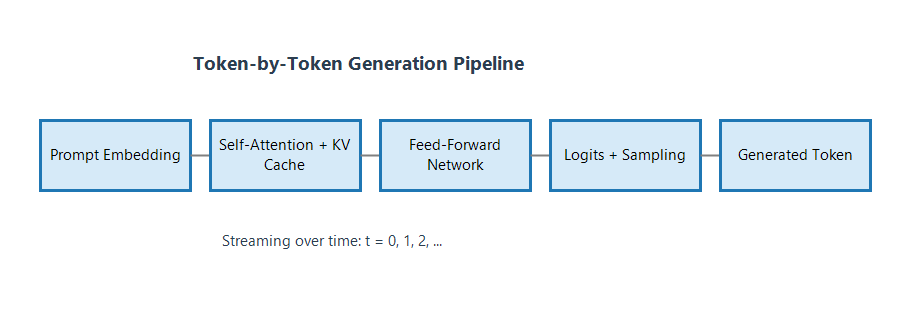
\includegraphics[width=0.85\textwidth]{token_generation_pipeline.png}
  \caption{Token-by-token generation pipeline with KV cache reuse and per-step sampling.}
  \label{fig:token_pipeline_en}
\end{figure}
Core properties:
\begin{itemize}
  \item \textbf{Latency scales with length:} Each decoded token triggers a full forward pass, so response time grows linearly with the number of generated tokens.
  \item \textbf{State reuse is critical:} KV cache reduces attention complexity from $O(n^2)$ to $O(n)$ per step, trading memory for compute.
  \item \textbf{Sampling is decoupled:} Temperature, top-$k$, nucleus sampling, and repetition penalties are applied to logits post-forward, enabling customized behaviors.
\end{itemize}

\subsection{Batching and pipelining}
Serving systems exploit batching and pipelining to increase hardware utilization:
\begin{itemize}
  \item \textbf{Static batching:} Merge requests with the same prompt length for joint prompt processing, maximizing tensor core throughput.
  \item \textbf{Dynamic batching:} Continuously merge ongoing decoding requests, inserting or removing sequences after each step while tracking offsets.
  \item \textbf{Pipeline parallelism:} Partition the model across GPUs; tokens flow through the pipeline stage by stage, reducing per-device memory footprint.
\end{itemize}
Schedulers must mitigate \emph{batch stragglers}: requests with vastly different generation lengths reduce utilization. Typical mitigations:
\begin{enumerate}
  \item Enforce maximum generation lengths or chunk long-form requests into smaller segments with retrieval augmentation;
  \item Prioritize high-SLA traffic with weighted fair queuing or shortest-remaining-time scheduling;
  \item Split warm-up (prompt) and hot (decode) phases into separated queues to tune policies independently.
\end{enumerate}

\subsection{Latency tuning and observability}
Meeting service-level objectives (SLOs) demands optimizations across the stack:
\begin{itemize}
  \item \textbf{Model kernels:} Fuse layer normalization, residual adds, and feed-forward operations; enable FlashAttention or fused MLP kernels to minimize memory traffic.
  \item \textbf{Runtime layer:} Employ asynchronous I/O, thread pools, and preallocated memory arenas to avoid allocator contention; log per-kernel latency histograms.
  \item \textbf{System layer:} Reduce network copies via zero-copy transports, colocate caching layers with inference pods, and isolate noisy neighbors in multi-tenant clusters.
\end{itemize}
Profilers such as NVIDIA Nsight Systems, PyTorch Profiler, or triton trace events reveal queueing delays, host-device copies, and underutilized kernels. Monitor P50/P95/P99 latencies continuously and adjust batch sizes or scheduling weights accordingly.

\section{Speculative Decoding and KV Cache Reuse}
\subsection{Algorithm mechanics}
Speculative decoding runs a lightweight draft model in parallel with the target model to reduce the number of expensive evaluations. The workflow:
\begin{enumerate}
  \item A draft model proposes a prefix of $k$ candidate tokens $\hat{x}_{t:t+k}$ using cached states.
  \item The target model validates the proposal token by token, checking acceptance criteria and streaming accepted tokens immediately.
  \item Accepted tokens reuse the draft model's KV cache; rejections trigger fallback decoding by the target model.
\end{enumerate}
Figure~\ref{fig:speculative_en} illustrates the validate-and-commit pattern in practice.
\begin{figure}[H]
  \centering
  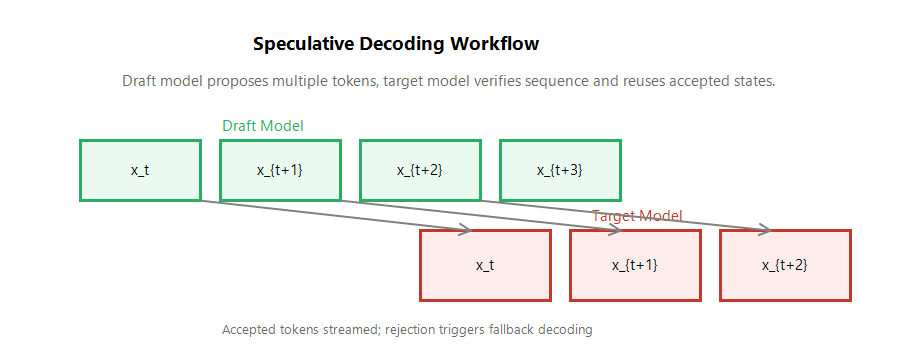
\includegraphics[width=0.85\textwidth]{speculative_decoding.png}
  \caption{Speculative decoding: the draft model proposes multiple tokens, the target model verifies and reuses accepted KV states.}
  \label{fig:speculative_en}
\end{figure}

\subsection{Acceptance rules and distribution alignment}
To preserve output fidelity, the target model checks each candidate token with a rejection-sampling style test. With target distribution $p_\theta$ and draft distribution $q_\phi$, the acceptance probability is
\begin{equation}
  \alpha(x) = \min\left(1, \frac{p_\theta(x \mid x_{<t})}{q_\phi(x \mid x_{<t})}\right).
\end{equation}
Practical considerations to maintain high acceptance:
\begin{itemize}
  \item Distill or fine-tune the draft model from the target model to keep distributions close.
  \item Apply temperature scaling or sharpen the draft logits to output conservative, high-probability tokens.
  \item Adapt the draft length $k$ per request based on observed acceptance rates and latency budgets.
\end{itemize}

\subsection{Sharing and managing KV cache}
Efficient cache sharing is crucial for realizing speedups:
\begin{itemize}
  \item \textbf{Unified layout:} Align hidden size, head count, and tensor precision so that draft KV tensors can be copied or referenced directly by the target model.
  \item \textbf{Lazy writes:} Mark cache blocks as ``validated'' without immediate copying; perform writes only when the token is accepted to avoid rollback overhead.
  \item \textbf{Batch-aware scheduling:} Interleave validation across requests so the target model stays saturated even when some sequences require fallback decoding.
\end{itemize}
Well-tuned speculative decoding offers $1.5$--$2.5\times$ throughput gains on popular 30B--70B models, especially when both models fit on a single GPU.

\subsection{Edge cases and safeguards}
\begin{itemize}
  \item \textbf{Long-context drift:} Periodically force synchronization tokens to keep the draft model aligned when decoding beyond training lengths.
  \item \textbf{High-diversity sampling:} Increase acceptance slack or shorten draft spans when using high temperature or nucleus sampling, which widens the draft-target gap.
  \item \textbf{Graceful degradation:} Automatically disable the draft path during overload, hardware failures, or when acceptance drops below a threshold.
\end{itemize}

\section{Model Quantization (4bit, 8bit, GPTQ, AWQ)}
\subsection{Foundations and trade-offs}
Quantization reduces memory footprint and bandwidth by mapping floating-point weights and activations to low-bit integer grids. For weights $w \in \mathbb{R}^n$,
\begin{equation}
  \tilde{w} = s \cdot \mathrm{clip}\!\left(\mathrm{round}\!\left(\frac{w}{s}\right), q_{\min}, q_{\max}\right),
\end{equation}
where $s$ is the scale and $[q_{\min}, q_{\max}]$ depends on bit width. Key trade-offs:
\begin{itemize}
  \item \textbf{Accuracy degradation:} Lower precision introduces quantization error; calibration or quantization-aware training mitigates loss.
  \item \textbf{Throughput benefits:} Less memory traffic improves effective FLOPs and power efficiency.
  \item \textbf{Engineering complexity:} Runtime kernels must decode INT4/INT8 tensors efficiently to avoid erasing speed gains.
\end{itemize}

\subsection{8-bit quantization (LLM.int8, SmoothQuant)}
INT8 is a safe compromise for production workloads:
\begin{itemize}
  \item \textbf{LLM.int8:} Splits high-variance rows to FP16 while quantizing the rest, preserving perplexity with minimal kernel changes.
  \item \textbf{SmoothQuant:} Jointly scales weights and activations to tame outliers, enabling fully INT8 transformer inference.
\end{itemize}
INT8 delivers roughly $2\times$ memory savings with negligible quality loss and integrates cleanly with server-grade GPUs.

\subsection{4-bit quantization and GPTQ}
INT4 cuts weight storage to one quarter of FP16 while posing steeper accuracy challenges. GPTQ (Gradient Post-Training Quantization) addresses this by fitting each layer's weights:
\begin{enumerate}
  \item Gather calibration activations to approximate the Hessian diagonal or gradient variance.
  \item Quantize columns sequentially, choosing the value that minimizes reconstruction error; propagate residuals to remaining columns.
  \item Allow mixed precision for sensitive columns or layers to cap perplexity regression.
\end{enumerate}
GPTQ requires no gradients from the original training run and works well for offline compression but demands careful calibration data selection.

\subsection{AWQ and activation-aware schemes}
AWQ (Activation-aware Weight Quantization) extends INT4 by preserving critical channels:
\begin{itemize}
  \item Estimate channel importance via activation sensitivity and allocate higher scaling factors or higher precision to important channels.
  \item Apply per-channel scaling in attention and MLP blocks, reducing error accumulation in long-context usage.
  \item Export metadata so inference engines can skip dequantization for low-impact channels.
\end{itemize}
In practice AWQ matches FP16 perplexity while retaining INT4 memory savings, and is widely supported by TensorRT-LLM, vLLM, and other runtimes.

\subsection{Quantization strategy comparison}
\begin{longtable}{p{3cm}p{3cm}p{4cm}p{4cm}}
\toprule
Method & Bit width & Highlights & Recommended use \\
\midrule
LLM.int8 / SmoothQuant & 8-bit & Minimal accuracy loss, channel-wise scaling & Production services requiring predictable quality \\
GPTQ & 4-bit & Post-training, second-order column fitting & Offline or edge deployments with calibration data \\
AWQ & 4-bit & Activation-sensitive, critical channel protection & Long-context or attention-heavy scenarios \\
QLoRA & 4-bit weights + 16-bit adapters & Quantized base with low-rank adaptation & Memory-efficient fine-tuning and serving \\
\bottomrule
\end{longtable}
Deployments often pair weight quantization with FP16 activations, selectively keeping attention output and final projection in higher precision to prevent saturation.

\section{Inference Frameworks (vLLM, TGI, Exllama)}
\subsection{vLLM: PagedAttention and continuous batching}
vLLM treats KV cache as paged virtual memory and introduces PagedAttention:
\begin{itemize}
  \item \textbf{Fragmentation-free KV cache:} Page tables remap cache blocks to consolidate fragmented memory across concurrent sessions.
  \item \textbf{Continuous batching:} Dynamically insert new requests into ongoing decode loops, maximizing GPU utilization under bursty traffic.
  \item \textbf{Unified APIs:} Drop-in compatibility with OpenAI-style endpoints and support for HF weights, TensorRT-LLM exports, and quantized checkpoints.
\end{itemize}
Advanced features such as speculative decoding, prefix caching, and LoRA merging make vLLM a strong base for multi-tenant inference clusters.

\subsection{Text Generation Inference (TGI)}
HuggingFace's TGI targets production readiness end to end:
\begin{itemize}
  \item \textbf{Optimized kernels:} Integrates FlashAttention, PagedAttention, and fused MLP kernels along with BetterTransformer fallbacks.
  \item \textbf{Orchestration:} Provides tensor parallelism, sharded loading, request routing, and rate limiting with Kubernetes-friendly deployment.
  \item \textbf{Ops tooling:} Exposes Prometheus metrics, structured logging, live config reloads, and model hot-swapping for high-availability services.
\end{itemize}
TGI pulls models directly from HuggingFace Hub, supports LoRA merging, on-demand LoRA loading, and integrates quantized artifacts without manual conversion.

\subsection{Exllama: Lightweight local inference}
Exllama specializes in 4-bit GPTQ models for consumer GPUs:
\begin{itemize}
  \item \textbf{Custom kernels:} Implements high-throughput INT4 matrix multiplication and tailored cache layouts optimized for GPTQ weight packs.
  \item \textbf{Memory efficiency:} Stores KV cache separately and streams weights to run 30B-class models on 12GB cards.
  \item \textbf{Accessible tooling:} Ships with Python bindings and lightweight front-ends for local assistants, offline experimentation, and privacy-sensitive use cases.
\end{itemize}
While Exllama lacks large-scale orchestration features, it excels where deployment simplicity and hardware constraints dominate.

\subsection{Choosing a serving stack}
Guidance for selecting frameworks:
\begin{itemize}
  \item Choose \textbf{vLLM} for peak throughput, speculative decoding, and multi-tenant scheduling.
  \item Choose \textbf{TGI} when production governance (monitoring, rate limiting, failover) is paramount.
  \item Choose \textbf{Exllama} for local inference, edge devices, or experimentation with 4-bit GPTQ checkpoints.
  \item Combine engines, e.g., run Exllama as a draft model and vLLM as the target model to unlock speculative decoding on limited hardware.
\end{itemize}

\section*{Operational recommendations}
\begin{itemize}
  \item Profile prompt, decode, and post-processing stages separately; track memory footprint alongside latency.
  \item Validate each optimization (speculative decoding, quantization, caching) with A/B tests capturing throughput, acceptance rates, and human evaluation scores.
  \item Calibrate framework-specific schedulers against traffic patterns, reserving headroom for bursty workloads and fallback paths.
\end{itemize}

\section*{Further reading}
\begin{itemize}
  \item Leviathan et al. ``Fast Inference from Transformers via Speculative Decoding.'' ICML, 2023.
  \item Frantar et al. ``GPTQ: Accurate Post-Training Quantization for Generative Pre-trained Transformers.'' NeurIPS, 2022.
  \item Lin et al. ``AWQ: Activation-aware Weight Quantization for LLM Compression and Acceleration.'' arXiv, 2023.
  \item Kwon et al. ``Efficient Memory Management for Large Language Model Serving with PagedAttention.'' arXiv, 2023.
  \item HuggingFace. ``Text Generation Inference: Scalable Production-ready LLM Serving.'' Technical Report, 2024.
\end{itemize}

\end{document}

